\begin{flushright} {\tiny {\color{gray} python\_codes/fieldstone\_141/text.tex}} \end{flushright}

%\lstinputlisting[language=bash,basicstyle=\small]{python_codes/fieldstone_141/keywords.ascii}

\begin{center}

\fbox{\textbf{\huge \color{teal} P}}
Codes at \url{https://github.com/cedrict/fieldstone/tree/master/python_codes/fieldstone_141}
\end{center}

\par\noindent\rule{\textwidth}{0.4pt}

%{\sl The python stone was developed in collaboration with Job Mos}. \index{contributors}{J. Mos}

%\par\noindent\rule{\textwidth}{0.4pt}
%%%%%%%%%%%%%%%%%%%%%%%%%%%%%%%%%%%%%%%%%%%%%%%%%%%%%%%%%%%%%%%%%%%%%%%%%%%%%%%%%%%%%%%%%%%%%%


The title of this \stone is voluntarily meant to be funny. 
Nobody calls what follows the 'Beaumont trick' but it has been 
prominent in many of his publications, all based on the \sopale code.
Let us look at the following figures from a few papers and focus on the 
initial temperature field.

\begin{center}
\fbox{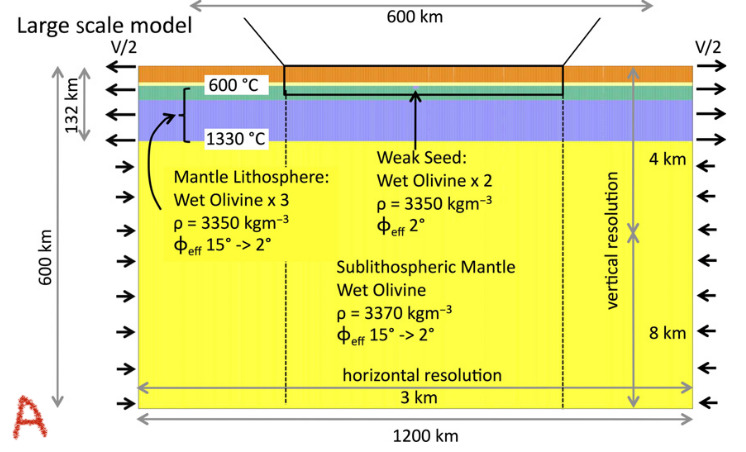
\includegraphics[width=8cm]{python_codes/fieldstone_141/images/albe15}}
\fbox{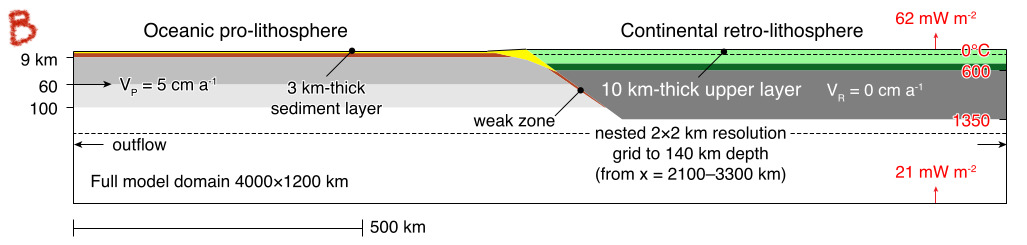
\includegraphics[width=8cm]{python_codes/fieldstone_141/images/bube17}}\\
\fbox{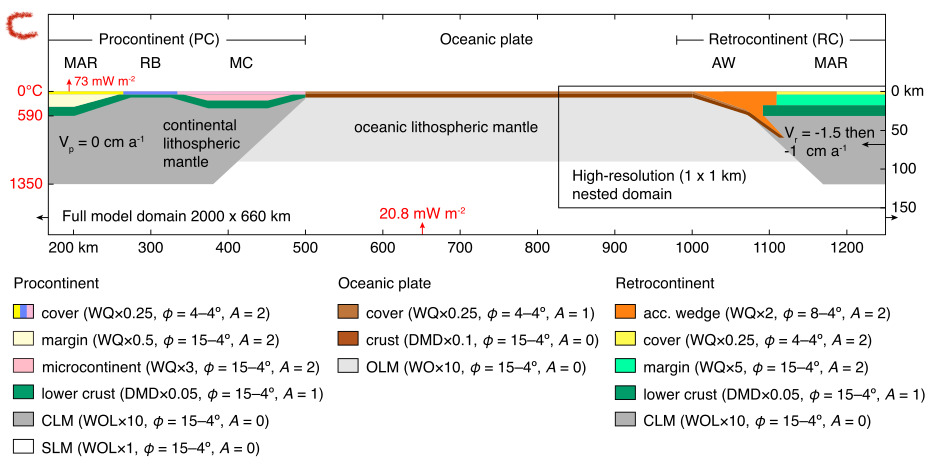
\includegraphics[width=8cm]{python_codes/fieldstone_141/images/bubj14}}
\fbox{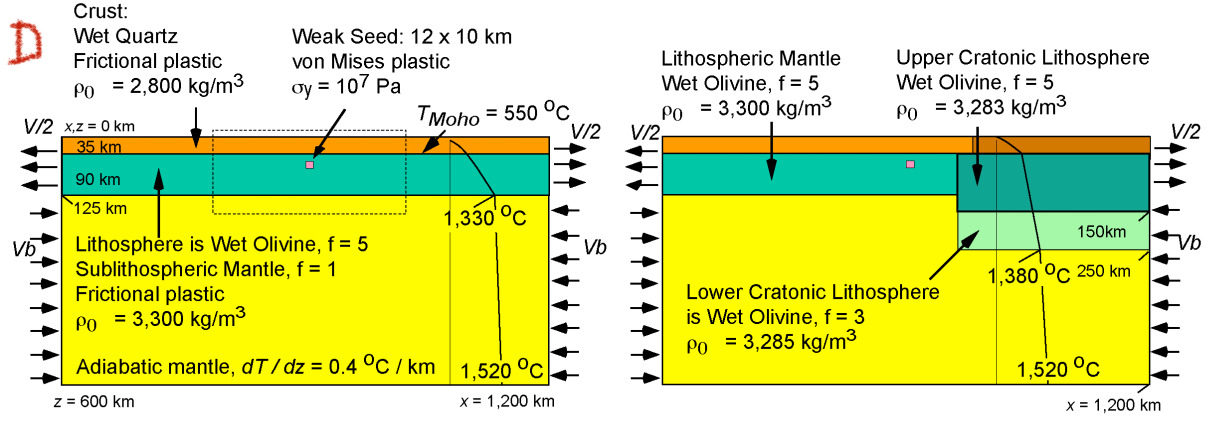
\includegraphics[width=8cm]{python_codes/fieldstone_141/images/hube11}}\\
\fbox{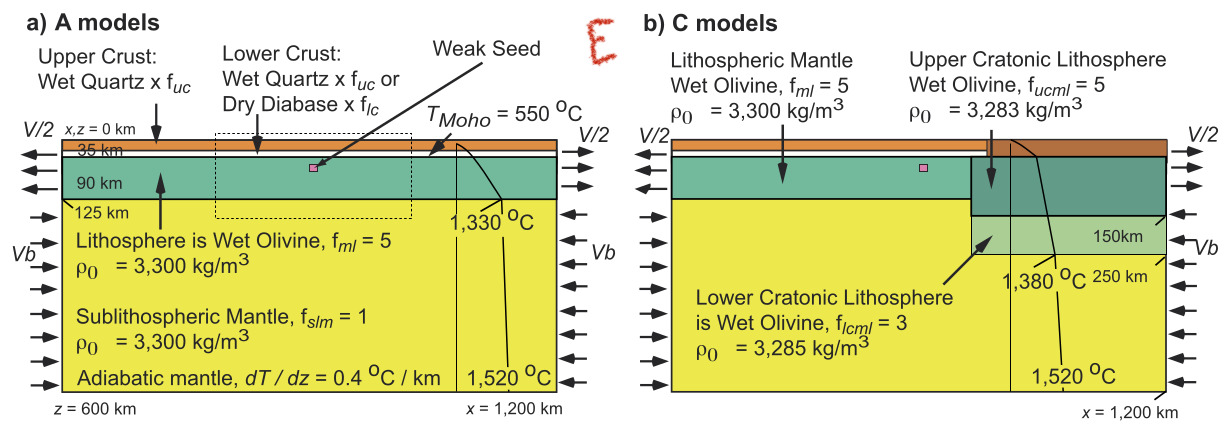
\includegraphics[width=8cm]{python_codes/fieldstone_141/images/hube14}}
\fbox{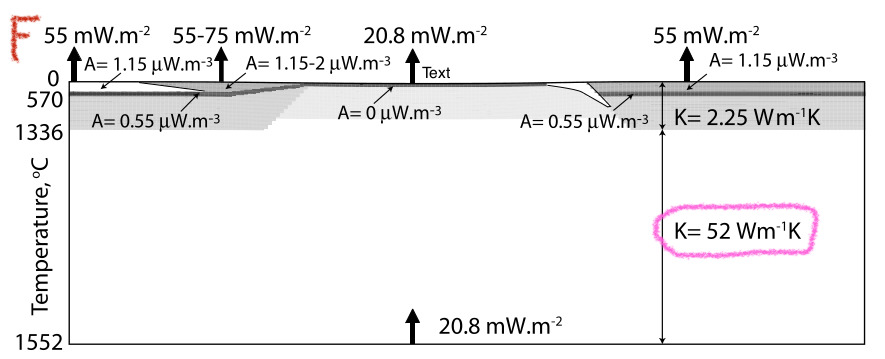
\includegraphics[width=8cm]{python_codes/fieldstone_141/images/wabj08}}\\
{\captionfont 
A: Taken from \textcite{albe15} (2015),
B: Taken from \textcite{bube17} (2017),
C: Taken from \textcite{bubj14} (2014).
D: Taken from \textcite{hube11} (2011),
E: Taken from \textcite{hube14} (2014),
F: Taken from \textcite{wabj08} (2008),
}
\end{center}

What is common to all is (aside from margins, cratons, sediment layers, etc ...) the presence 
of a crust, a lithosphere and a mantle. 
The temperature at the top of the model is $0~\si{\celsius}$, $500~\si{\celsius}$ at the base of the 
crust, $1330-1380~\si{\celsius}$ at the base of the lithosphere (it depends on its thickness), 
and on some of the figures we see that the temperature is $1234~\si{\celsius}$.

In between these depths the geotherm is linear (maybe parabolic in the crust where heat production
is present, but not too relevant here).

At this stage it is worth noting that at the base of the model a heat flux value is prescribed
(i.e. a Neumann boundary condition) of about $21~\si{\milli\watt\per\square\meter}$.

Another point worth noticing is the very large value of the heat conductivity 
$k=52~\si{\watt\per\meter\kelvin}$
of the mantle in \textcite{wabj08} (2008) (also in \textcite{wabj08b,wabj08c} - not shown here).
Indeed, we can look at the table of properties of all materials in the paper:

\begin{center}
\fbox{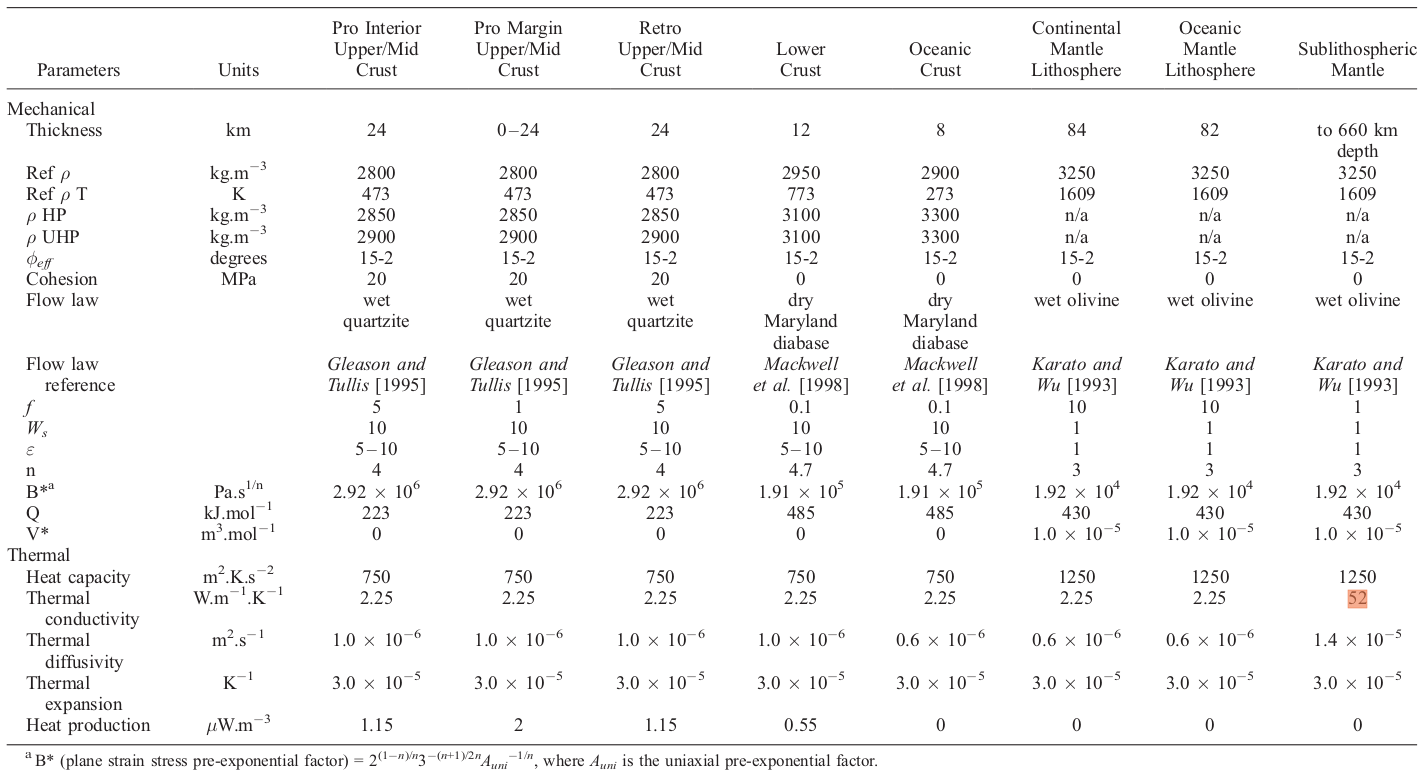
\includegraphics[width=13cm]{python_codes/fieldstone_141/images/wabj08-2}}\\
{\captionfont Taken from \textcite{wabj08} (2008).}
\end{center}

The purpose of this \stone is to answer these two questions: why did the authors set the 
conductivity of the mantle to such high values and why did they use heat flux boundary conditions?

In what follows we'll focus for simplicity 
on the setup of \textcite{hube11} (2011): a 35km crust, a 90km lithosphere, 
a 600km deep domain, with no variation in the horizontal direction. 


%------------------------------------------------------------------------------
\subsubsection*{Remarks about the code}

The first obvious thing to be mentioned is that this is inherently a 1D problem.
However, for practical reasons I have reused an existing 2D code. As such, 
we need to specify a lateral extent $L_x$ to the domain which can be only a 
few kilometers. 

The code is a FEM code relying on bi-linear elements $Q_1$. Both 
Dirichlet and Neumann boundary conditions are implemented. 
Before we use it to investigate the problem highlighted above, we need to 
make sure it works as intended, i.e. we need to carry out benchmarks.

Each element is assigned a heat conductivity $k$, heat capacity $C_p$ and density $\rho$.

The timestep value is computed by means of a CFL condition for diffusive 
processes, i.e. $dt=0.75*\min(h_x,h_y)^2/\max(\kappa)$ where
$h_x,h_y$ is the size of an element, and $\kappa$ is the heat diffusivity
given by $\kappa=k/\rho C_p$.

how is q nodal computed

%------------------------------------------------------------------------------
\subsubsection*{benchmark \#1}

The domain is $5\times 100~\si{\km}$. 
Temperature boundary conditions are imposed at the top and bottom with 
$T_{top}=0\si{\celsius}$
and $T_{bottom}=100\si{\celsius}$.
The initial temperature $T(x,y,t=0)$ is set to $T_{top}$.



%------------------------------------------------------------------------------
\subsubsection*{benchmark \#2}

The domain is $5\times 100~\si{\km}$. 
Temperature boundary conditions are imposed at the top with 
$T_{top}=0\si{\celsius}$
and a heat flux is prescribed at the bottom 
$q_{bottom}=0.03~\si{\watt\per\square\meter}$.
The initial temperature $T(x,y,t=0)$ is set to $T_{top}$.

The expected steady state solution is such that the temperature is 
$T(x,y=L_y,t)=T_{top}$ and $q_y(x,y,t)=q_{bottom}$. 
Since then $|q_y|=k \Delta T/L_y$, then we expect a temperature at the
bottom of $60~\si{\celsius}$.

\begin{center}
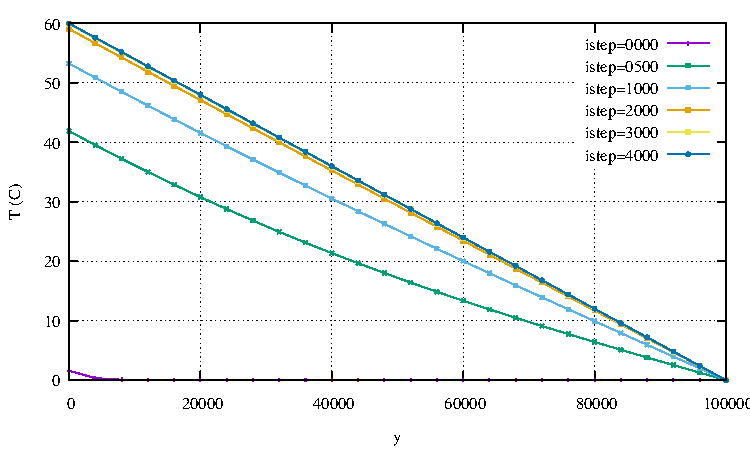
\includegraphics[width=8cm]{python_codes/fieldstone_141/results/test2/temperature}
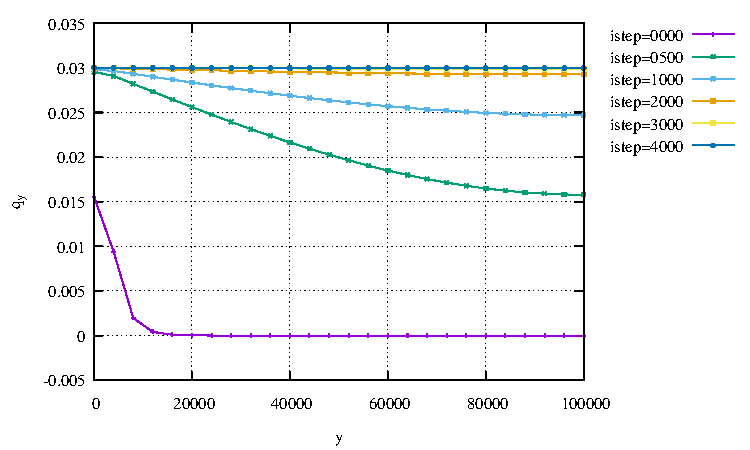
\includegraphics[width=8cm]{python_codes/fieldstone_141/results/test2/heat_flux}
\end{center}

\begin{center}
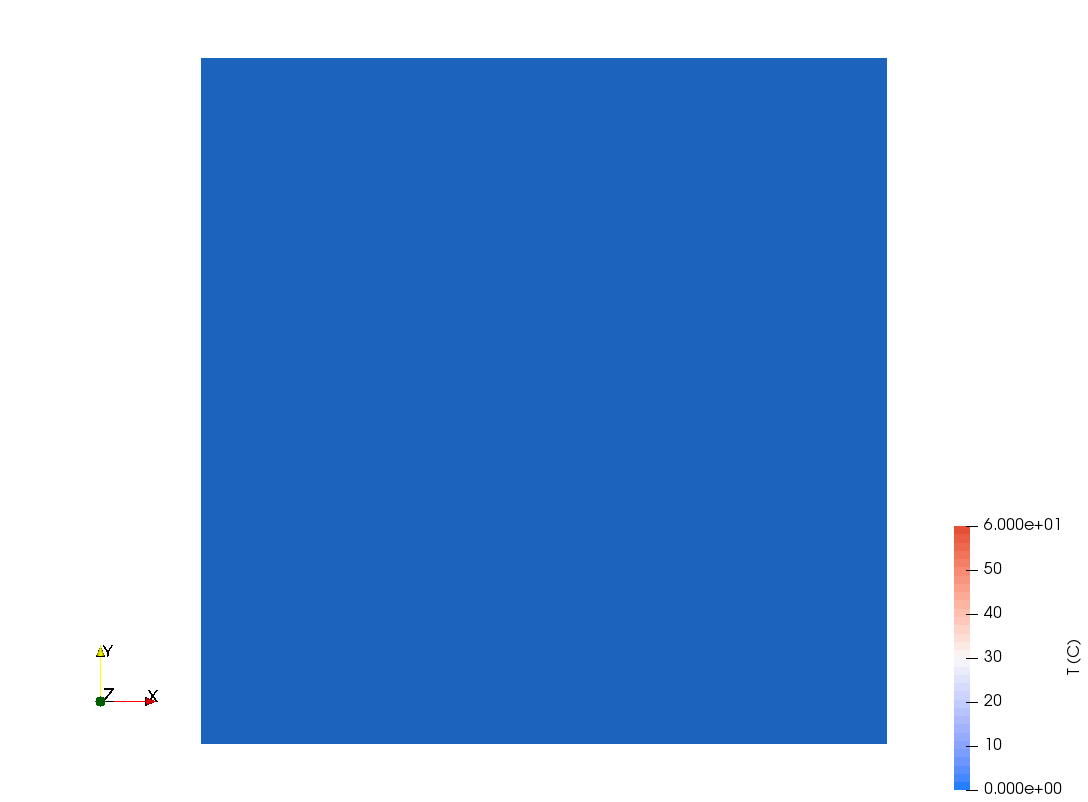
\includegraphics[width=5cm]{python_codes/fieldstone_141/results/test2/T0000}
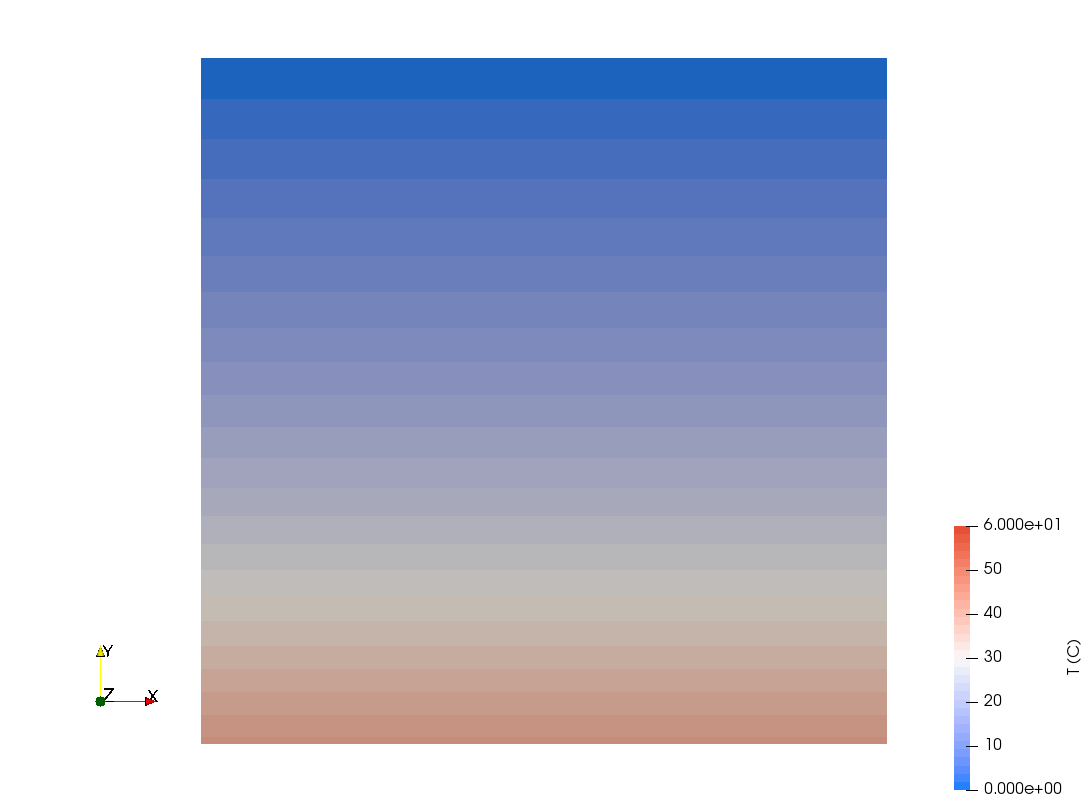
\includegraphics[width=5cm]{python_codes/fieldstone_141/results/test2/T0500}
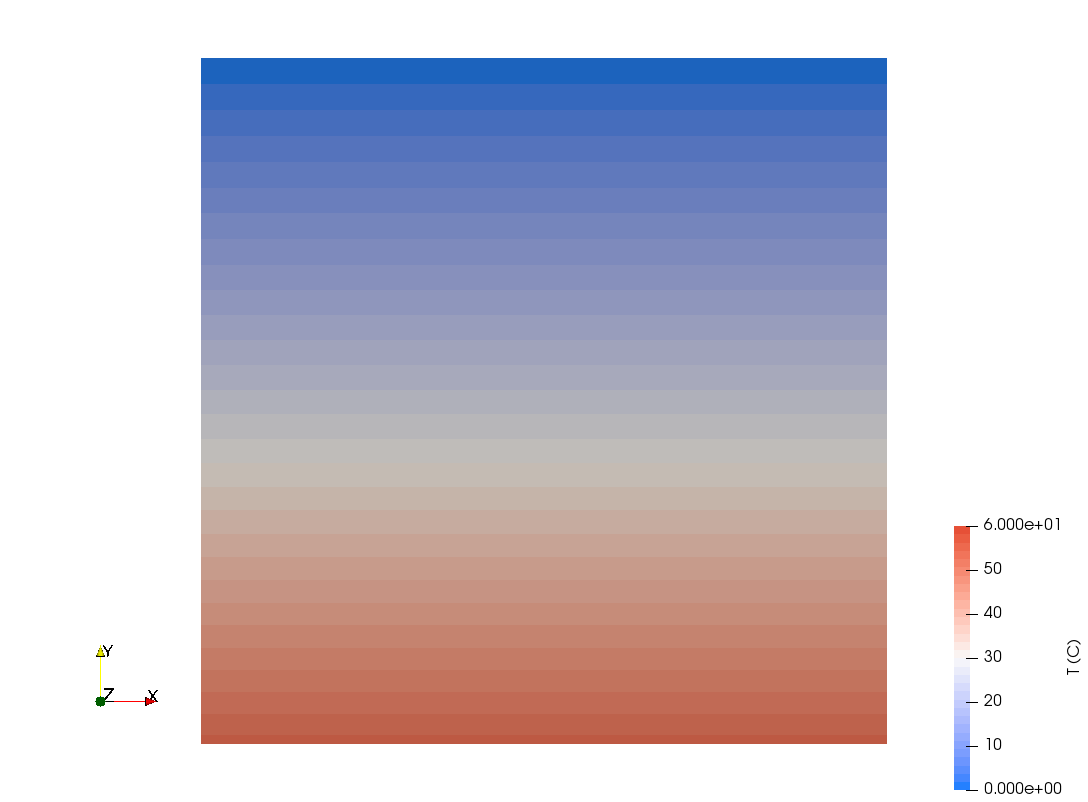
\includegraphics[width=5cm]{python_codes/fieldstone_141/results/test2/T1000}\\
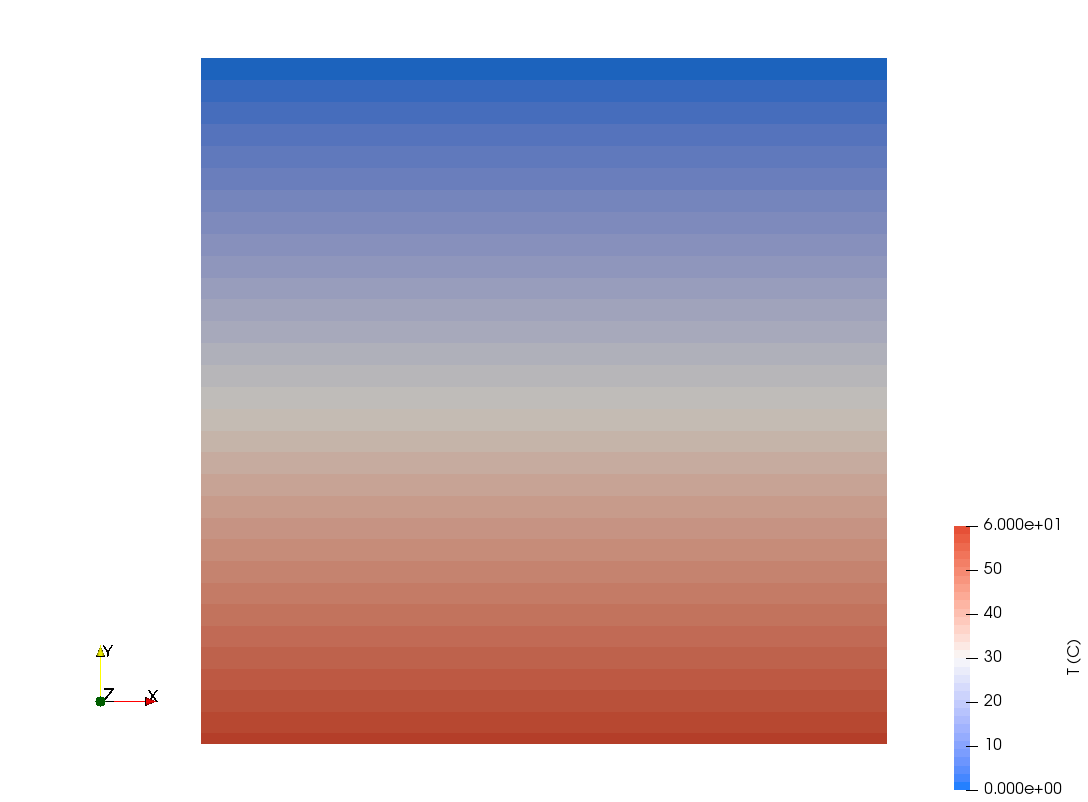
\includegraphics[width=5cm]{python_codes/fieldstone_141/results/test2/T2000}
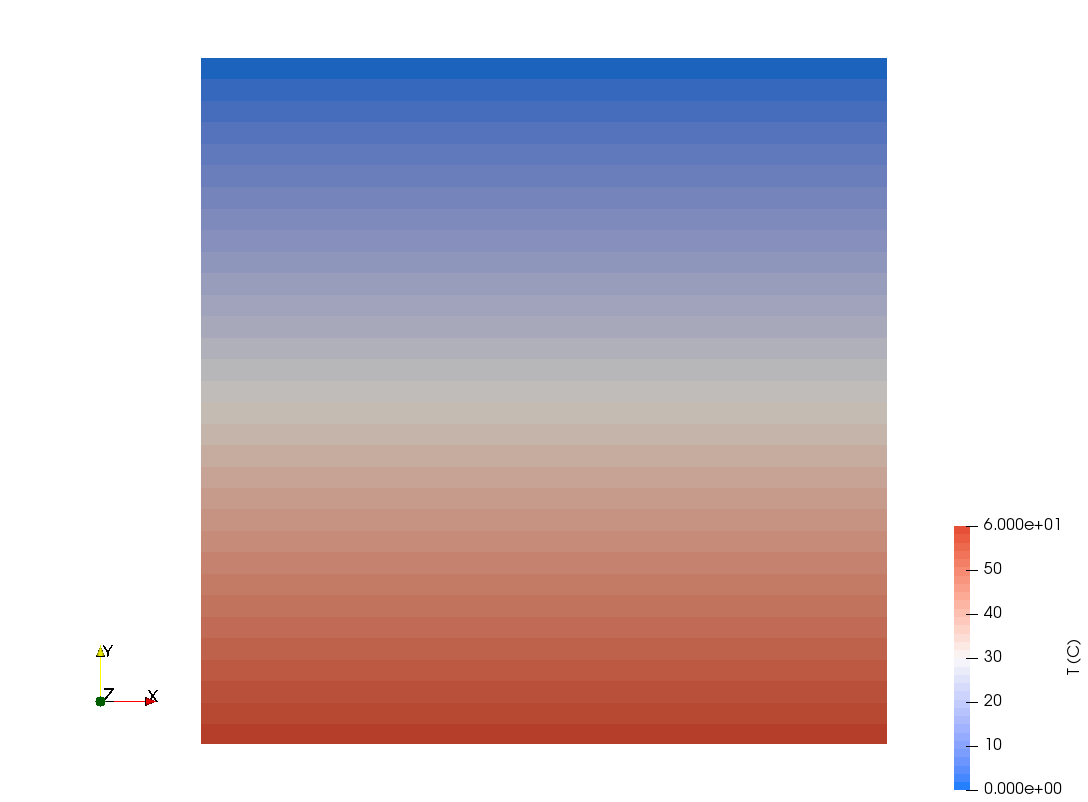
\includegraphics[width=5cm]{python_codes/fieldstone_141/results/test2/T3000}
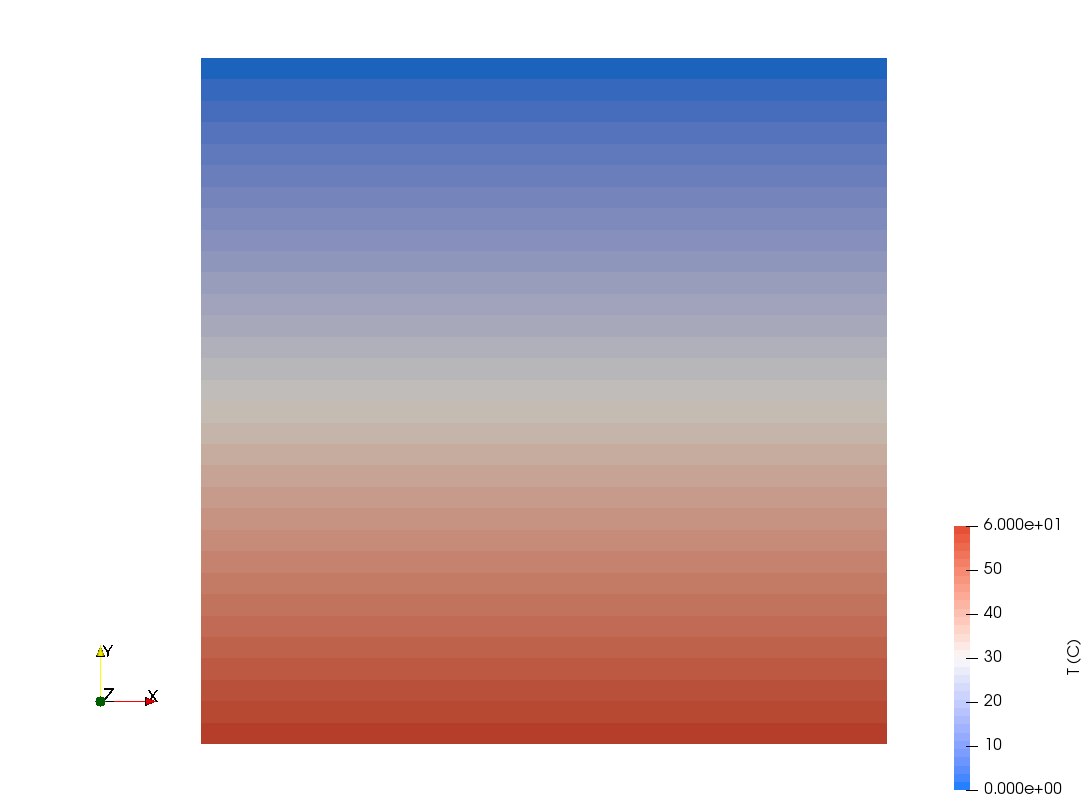
\includegraphics[width=5cm]{python_codes/fieldstone_141/results/test2/T4000}\\
{\captionfont Time evolution of the temperature field.}
\end{center}








